\chapter{Generating Random Variables}

\section{Generating Discrete Random Variables}

Main component of a simulation study is the ability to generate random number, where a random number represents the value of random variable uniform
distribution on $(0,1)$.
\subsection{Pseudorandom Number Generation}
Random numbers were originally either manually or mechanically generated, by using spinning wheels or dice rolling or card shuffling
but the modern approach is to use a computer to successively generate pseudorandom numbers.

One of the common approaches to generate pseudorandom numbers starts with an initial value $x_0$, called seed, and then recursively computes
successive values $x_n, n\ge1$, by letting
\begin{equation}
	\label{MCM}
	x_n = a x_{n-1} \text{ modulo } m
\end{equation}
where $a$ and $m$ are given positive integers, and where \Cref{MCM} means that $ax_{n-1}$ is divided by  $m$ and remainder is taken as the
value of $x_n$. Thus, each value of $x_n$ is either $0,1, \ldots, m-1$ and the quantity $x_n / m$ is Pseudorandom number and follows
an approximation to the value of a uniform $(0,1)$ random variable.

The approach specified by \Cref{MCM} to generate random numbers is called the Multiplicative Congruential Method.

Another method is
\[
	x_n = (a x_{n-1}+c) \text{ modulo } m
\]
this method is known as \textit{Mixed Congruential Generators} or \textit{Linear congruential Generations (LCGs)} where $c$ is a non-negative integer.

\subsection{The Inverse Transform Method}
Suppose we want to generate the value of a discrete random variable $X$ having probability mass function
\[
	P(X=x_i)=p_i, \ i = 0,1, \ldots , \ \sum_ip_i =1
\]
To do this, we generate a random number from a uniform distribution $(0,1)$ $U$, and set
\[
	X=
	\begin{cases}
		x_0 \text{ if } U<p_0                                         \\
		x_1 \text{ if } p_0\le U\le p_0+p_1                           \\
		\vdots                                                        \\
		x_j \text{ if } \sum_{i=0}^{j-1}p_i\le U\le \sum_{i=0}^{j}p_i \\
		\vdots
	\end{cases}
\]
Since, for $0<a<b<1, P(a\le U<b) = b-a$, we have,
\[
	P(X=x_j)=P\left( \sum_{i=0}^{j-1}p_i\le U< \sum_{i=0}^{j}p_i \right) = p_j
	.\]
So, $X$ has the desired distribution.

\begin{example}[Bernoulli Distribution]
	Let, $X\sim Ber(p)$ where p is success probability  i.e.  $P(X=0)= 1-p$ and  $P(X=1)=p$ and $0\le p \le 1$.
	Then, to generate $X$ we first generate $U \sim U[0,1]$ then, we set

	\[
		X=
		\begin{cases}
			1, \text{ if } U\le p \\
			0, \text{ if } U> p
		\end{cases}
	\]
	Hence, $X$ follows Bernoulli Distribution with the parameter $p$.\\
	\textbf{Algorithm for Inverse Transform Algorithm for Generating Bernoulli Distribution:}\\
	STEP 1: Generate a random variable $U\sim U[0,1]$.\\
	STEP 2: If $U\le p$ set $X=1$ or set  $X=0$. \\
	STEP 3: Go to  STEP 1.

	\begin{figure}[H]
		\centering
		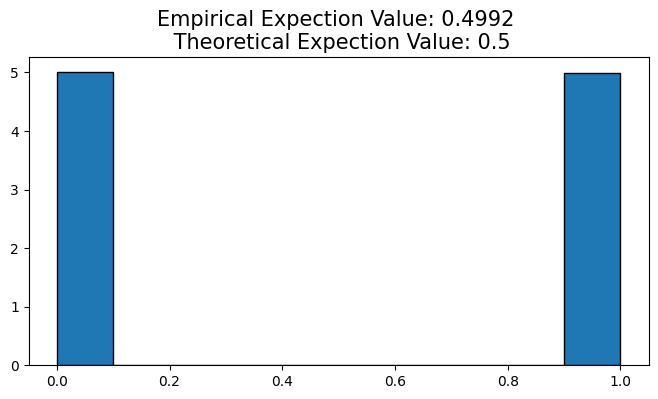
\includegraphics[width=0.6\textwidth]{ber_ITA.png}
		\caption{Inverse Transform method for generating  Bernoulli random numbers with $p=0.5$}
	\end{figure}
\end{example}

\begin{example}[Binomial Distribution]
	Let, $X\sim Bin(n,p)$ then,  $X$ has probability mass function
	\[
		f(r) = P(X=r) = {n\choose r}p^{r}(1-p)^{n-r},\  i = 1,2, \ldots
	\]
	The generation of $X\sim Bin(n,p)$ by Inverse Transform Algorithm can be tedious. We can use the relation between Binomial and Bernoulli distribution.
	If $x_i \sim Ber(p), \forall i = 1,2, \ldots, n$ then, $\sum_{i=1}^{n} x_i\sim Bin(n,p)$.

	Hence, by generating $x_i$ $n$ independent random variable from Bernoulli distribution and summing them we get binomial distribution
	\begin{figure}[H]
		\centering
		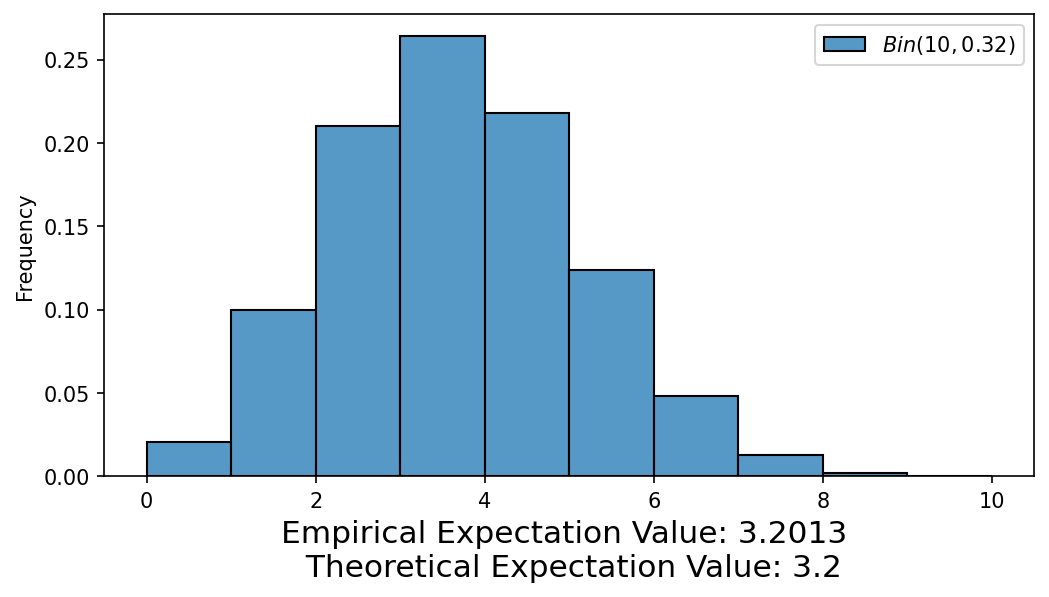
\includegraphics[width=0.6\textwidth]{images/bin_ITA.png}
		\caption{Generating  binomial random numbers with $n=10$ and  $p=0.32$}
	\end{figure}
\end{example}

\section{Generating Continuous Random Variables}

\subsection{The Inverse Transform Algorithm}
To generate Continuous random variables The Inverse Transform Algorithm is very important method. It is based on a following theorem.
\begin{theorem}
	\label{ITA theorem}
	Let $U$ be a uniform  $(0,1)$ random variable. For any continuous distribution function  $F$ the random variable  $X$ defined by
	\[
		X=F^{-1}(U)
	\]
	has distribution $F$.
\end{theorem}
\begin{proof}
	Let, $F_X$ denote the distribution function of  $X=F^{-1}(U)$. Then,
	\begin{align*}
		F_X(x) & = P(X\le x)         \\
		       & = P(F^{-1}(U)\le x) \\
	\end{align*}
	Since, $F$ is a cumulative distribution function it follows that $F(x)$ is monotonic increasing function of  $x$ and range of  $F(x)$ is  $(0,1)$.
	Then,
	\begin{align*}
		F_X(x) & = P\left(F\left(F^{-1}(U)\right)\le F(x)\right) \\
		       & = P(U\le F(x))                                  \\
		       & = F(x) \text{ since $U\sim U(0,1)$ }
	\end{align*}
\end{proof}

The above theory tells us we can generate a random variable $X$ from the continuous distribution function  $F$ by generating a random number $U\sim U(0,1)$
and setting $X=F^{-1}(U)$.

\begin{example}[Exponential Distribution]
	\label{exponential distribution}
	Suppose we want to generate a random variable $x\sim Exp(\lambda)$, then its probability density function is
	\[
		f(x) = \lambda e^{-\lambda x}.
	\]
	Hence, The cumulative distribution function is,
	\[
		F(x) = 1-e^{\lambda x}
	\]
	if we let $x=F^{-1}(u)$, then,
	\begin{align*}
		u   & =F(x)=1-e^{-\lambda x}       \\
		1-u & = e ^{-\lambda x}            \\
		x   & = - \frac{\ln(1-u)}{\lambda}
	\end{align*}

	Hence, we can generate an exponential random variable with parameter 1 by generating a uniform $(0,1)$ random number $U$ and then setting
	\[
		X = F^{-1}(U) = -\frac{\ln(1-U)}{\lambda}.
	\]
	We see that if $U\sim U(0,1)$ then also $1-U\sim U(0,1)$ thus  $\ln(1-U)$ has the same distribution as  $\ln(U)$ so,
	\[
		X = F^{-1}(U) = -\frac{\ln(U)}{\lambda}.
	\]
	will also work. If we use second expression then the algorithm will take less computing power hence less time.
	\begin{figure}[H]

		\centering
		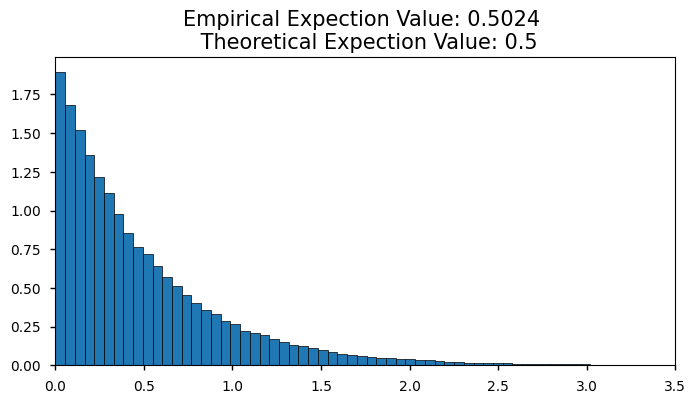
\includegraphics[width=0.6\textwidth]{images/exp_ITA.png}
		\caption{Inverse Transform method for generating $Exp(2)$}
	\end{figure}
\end{example}
\begin{example}[Gamma Distribution]
	Let $X\sim G(n,\lambda)$ Then, its probability  mass function is given by,
	\[
		f(x) = \frac{1}{\Gamma(n)}\lambda^{n}x^{n-1}e^{-\lambda x}
	\]

	We know if $X_i\sim Exp(\lambda) \forall i = 1,2, \ldots ,n$ then  $Y=\sum_i X_i \sim G(n,\lambda)$. As,

	\begin{align*}
		M_{Y}(t) = E \left[ e^{tY} \right] = E\left[ e^{\sum_{i=1}^{n} X_it  }\right] & = E\left[ \prod_{i=1}^{n} e^{X_it} \right]                                                \\
		                                                                              & =\prod_{i=1}^{n} E\left[  e^{X_it} \right] \text{ As all $X_i$ are independent }          \\
		                                                                              & = \prod_{i=1}^{n}\frac{\lambda}{\lambda-t} = \left( \frac{\lambda}{\lambda-t} \right)^{n}
	\end{align*}

	Then, Generating  $n$ number of $X_i\sim Exp(\lambda)$
	and summing them we can easily generate a random variable which follows gamma distribution
	\begin{figure}[H]

		\centering
		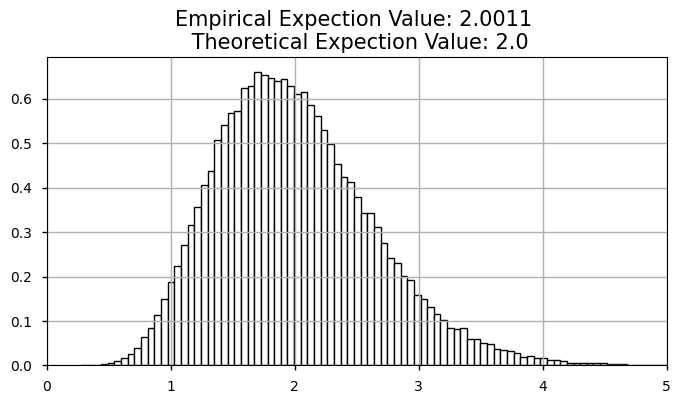
\includegraphics[width=0.6\textwidth]{images/gamma_ITA.png}
		\caption{$G(10,5)$ generated by summing of $Exp(5)$}
	\end{figure}
\end{example}

\subsection{Accept - Reject Method}
The accept–reject method is useful when it is difficult to directly simulate $f(x)$ but we can generate another density $g(x)$ such that $f(x)/g(x)$
is uniformly bounded and it is much easier to simulate $g(x)$. We simulate  $X$ from  $g$, and retain it or toss it according
to a probability proportional to $f(x)/g(x)$.
Because an $X$ value is either retained
or discarded, depending on whether it passes the admission rule, the method is called
the accept–reject method. The density $g(x)$ is called the envelope density.

The method proceeds as follows, \\
STEP 1: Find a density $g$ and a finite constant  $c$ such that  $\frac{f(x)}{g(x)}\le c \ \forall x$.\\
STEP 2: Generate $X\sim g$.\\
STEP 3: Generate  $U\sim U(0,1)$, independent of  $X$. \\
STEP 4: Retain this generated value  $X$ if  $U\le \frac{f(x)}{cg(x)}$.\\
STEP 5: Repeat the same until the required number of $n$ values of  $X$ has been obtained.\\

The following theorem supports the method.
\begin{theorem}
	Let $X\sim g$, and  $U$, independent of, be a distributed as $U[0,1]$. Then the conditional density of $X$ given that
	$U\le \frac{f(X)}{cg(X)}$ is $f$.
\end{theorem}
\begin{proof}
	Denote the CDF of $f$ by $F$. Then,
	\begin{align*}
		P\left( X\le x|U\le \frac{f(X)}{cg(X)} \right) & = \frac{P\left( X\le x, U\le \frac{f(X)}{cg(X)} \right)}{P\left( U\le \frac{f(x)}{cg(x)} \right)}                            \\
		                                               & = \frac{\int_{-\infty}^{x}\int_{0}^{\frac{f(t)}{cg(t)}}g(t)dudt}{\int_{-\infty}^{\infty}\int_0^{\frac{f(t)}{cg(t)}}g(t)dudt} \\
		                                               & = \frac{\int_{-\infty}^{x}f(t)dt}{\int_{-\infty}^{\infty}f(t)dt} = \frac{F(x)}{1}= F(x).
	\end{align*}
\end{proof}

\begin{example}[Generating a Normal Random Variable]
	\label{generate normal}
	To generate a standard normal variable $Z$ i.e. $Z\sim N(0,1)$, note first that the absolute value of  $Z$ has probability density function
	\begin{equation}
		\label{abs std normal}
		f(x) = \frac{2}{\sqrt{2\pi}}e^{- \frac{x^{2}}{2}} \ 0\le x \le \infty.
	\end{equation}
	Then, we can choose $g$ as the exponential density function with mean 1 i.e.
	\[
		g(x) = e^{-x}\ 0\le x\le \infty
	\]
	Now,
	\[
		\frac{f(x)}{g(x)} = \sqrt{\frac{2}{\pi}} e^{x-\frac{x^{2}}{2}}
	\]
	and so the maximum value of $f(x)/g(x)$ occurs at the value of $x$ that maximize $x-x^2 /2$ hence $x=1$ so we take
	\[
		c = \max_x \frac{f(x)}{g(x)} = \frac{f(1)}{g(1)} = \sqrt{\frac{2e}{\pi}}.
	\]
	Now,
	\[
		\frac{f(x)}{cg(x)} = \exp\left( x-\frac{x^2}{2}-\frac{1}{2} \right) = \exp\left( \frac{-(x-1)^2}{2} \right)
	\]
	Then, its follows that we can generate the absolute value of a standard normal random variable as follows: \\
	STEP 1: Generate $X\sim Exp(1)$. \\
	STEP 2: Generate $U\sim U(0,1)$, independent of $X$.\\
	STEP 3: If  $U\le \exp\left( -(X-1)^2 /2 \right)$, retain  $X$, Otherwise, return to Step 1.\\

	Once, we have simulated a random variable $X$ having density function as in
	\Cref{abs std normal} we can obtain a standard normal $Z$ by letting
	$Z$ be equally likely to be either  $X$ or  $-X$.
	In Step 3, the value $X$ is accepted if  $U\le \exp\left( -(X-1)^2 /2 \right)$, which is equivalent to $- \ln U\ge (X-1)^2 /2$.
	However, in \Cref{exponential distribution} we have seen that $-\ln{U}\sim Exp(1)$ When $U\sim U(0,1)$.

	So, summing up, we can generate the standard normal random variable $Z$ as follows:\\
	STEP 1: Generate independent $X_1, X_2\sim Exp(1) $\\
	STEP 2: If $X_2\ge (X_1-1)^2 /2$ retain $X_1$. Otherwise, return to Step 1.\\
	STEP 3: Generate $U\sim U(0,1)$ and set,
	\begin{eqnarray*}
		Z=
		\begin{cases}
			X_1 \text{ if } U\le \frac{1}{2}, \\
			X_1 \text{ if } U> \frac{1}{2}.
		\end{cases}
	\end{eqnarray*}

	\begin{figure}[H]

		\centering
		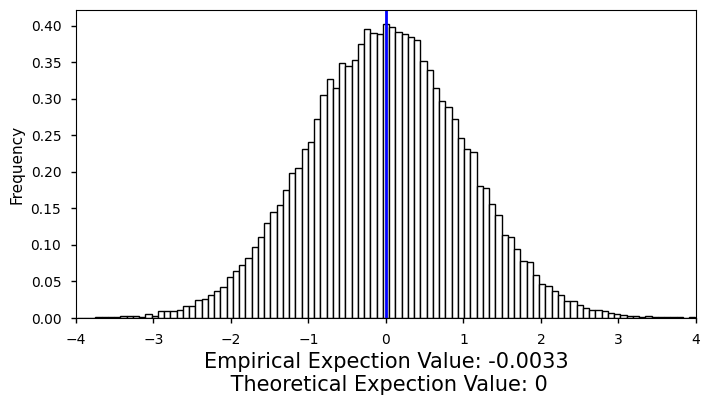
\includegraphics[width=0.6\textwidth]{images/nor_AR.png}
		\caption{Generating $N(0,1)$ with Accept - Reject method}
	\end{figure}

	If we want to generate normal random variable to have mean $\mu$  and variance $\sigma^2 $, just take $\mu +\sigma Z $.
\end{example}

\begin{example}[Generating Beta Distribution]
	\label{generate beta}
	If $\alpha$ and  $\beta $ are both getter then 1, then Beta density is uniformly bounded and its maximum attain at
	$\frac{\alpha-1}{\alpha+\beta-2}$. As a result the $U[0,1]$ density can be served as an envelope density for generating such Beta distribution by using accept-reject method.
	Precisely, generate $U$, $X\sim U[0,1]$ (independently), and retain the value if
	$U\le \frac{f(X)}{\sup_x f(X)}$, where,
	\[
		f(X)=\frac{\Gamma(\alpha+\beta)}{\Gamma(\alpha)\Gamma(\beta)}x^{\alpha-1} (1-x)^{\beta-1}, 0 < x< 1.
	\]
	Because
	\[
		\sup_x f(X) = f\left( \frac{\alpha-1}{\alpha+\beta-2} \right) = \frac{\Gamma(\alpha+\beta)}{\Gamma(\alpha)\Gamma(\beta)}\frac{(\alpha-1)^{\alpha-1} (\beta-1)^{\beta-1} }{(\alpha+\beta-2)^{\alpha+\beta-2} }
	\]
	The algorithm finally works out as follows:\\
	STEP 1: Generate independent $U,X \sim U[0,1]$.\\
	STEP 2: Retain the value $X$ if,
	\[
		U \le \frac{X^{\alpha-1} (1-X)^{\beta -1} (\alpha+\beta-2)^{\alpha+\beta-2} }{(\alpha-1)^{\alpha-1} (\beta-1)^{\beta-1} }.
	\]
	Otherwise, return to STEP 1.

	\begin{figure}[H]
		\centering
		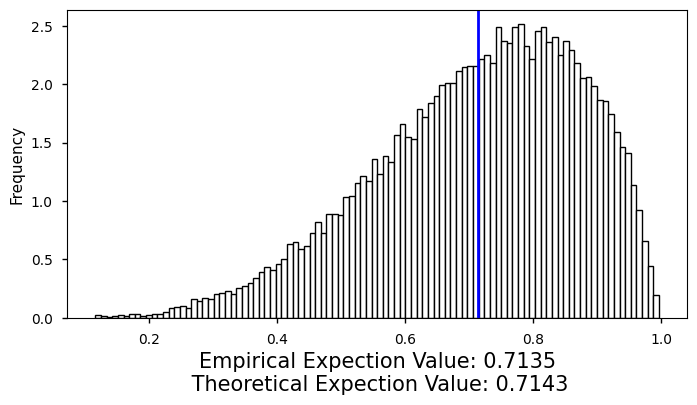
\includegraphics[width=0.6\textwidth]{images/beta_AR.png}
		\caption{Generating Beta(5,2) with accept-reject method}
		\label{Beta 5 2}
	\end{figure}
\end{example}

An issue about an accept-reject method is the acceptance rate.
Our goal make it as large as possible to increase the efficiency of the method.
This can be achieved by choosing $c$ to be smallest possible number, described in the result bellow.
\begin{theorem}[Acceptance Rate]
	For an accept-reject scheme, the probability that an $X\sim g$ is acceded is  $\frac{1}{c}$,
	and is maximized when $c$ is chosen to be $c=\sup_x\frac{f(x)}{g(x)}.$
\end{theorem}
\begin{proof}
	\begin{align*}
		P\left( U \le \frac{f(x)}{cg(x)} \right) & = \int_{-\infty}^{\infty} \int_{0}^{\frac{f(x)}{cg(x)}} g(t) du dt                                           \\
		                                         & = \int_{-\infty}^{\infty} \frac{f(t)}{cg(t)}g(t)dt = \int_{-\infty}^{\infty} \frac{f(t)}{c}dt = \frac{1}{c}.
	\end{align*}
	Because any $c$ that can be chosen must be at least as large as $\sup_x\frac{f(x)}{g(x)}$
	, obviously $1/c$ is maximized by choosing $c=\sup_x\frac{f(x)}{g(x)}.$
\end{proof}

In the \Cref{generate normal} for $N(0,1)$ the acceptance rate is $\sqrt{\frac{\pi}{2 e}} = 0.7601$.
And in the \Cref{generate beta} for Beta(5,2) the acceptance rate is 0.4069

\subsection{Bivariate Techniques}
Let $X$ and $Y$ be independent slandered normal random variable and let $R$ and $\theta$
denote the polar coordinates of vector $(X,Y)$. That is,
\begin{align*}
	R^{2}       & = X^{2} + Y^2 \\
	\tan \theta & = \frac{Y}{X}
\end{align*}

Since $X$ and $Y$ are independent, their joint density is the product of their individual densities and thus given by
\begin{align*}
	f(x,y) & = \frac{1}{\sqrt{2\pi}} e^{-x^{2}/2 } \frac{1}{\sqrt{2\pi}} e^{-y^{2}/2 } \\
	       & = \frac{1}{2\pi} e^{-(x^{2}+y^{2})/2}
\end{align*}
To determine the joint density of $R^{2} $ and $\Theta$ - call it $g(d,\theta)$ we make the change of variables
\[
	d=x^{2}+y^{2}, \ \  \theta=\tan^{-1}\left( \frac{y}{x} \right)
\]
Then the joint density function of $d $ and $\Theta$ is,

\begin{align*}
    \label{jacobian transformation}
    g(d,\theta) &= |J| f(x,y) \\ 
                &= |J| \frac{1}{2\pi} e^{-(x^{2}+y^{2})/2} \numberthis
\end{align*}
where,
\[
	J =
	\begin{vmatrix}
        \frac{\partial x}{\partial t} & \frac{\partial x}{\partial \theta} \\[1ex]
		\frac{\partial y}{\partial t} & \frac{\partial y}{\partial \theta} \\
	\end{vmatrix} = \frac{1}{2}.
\]
Then, replacing the value of $ x = \sqrt{d}\sin(\theta)  $ and $ y=\sqrt{d}\cos(\theta) $ in \Cref{jacobian transformation} we get,
\begin{equation}
	g(d,\theta) = \frac{1}{2}\frac{1}{2\pi} e^{-d/2},\ \ \ 0< d<\infty, 0<\theta<2 \pi.
\end{equation}

As $g(d,\theta)$ is equal to product of the product of $Exp(1/2)$ density and $U(0,2 \pi)$, it follows that,\\
$R^{2}$ and $\Theta$ are independent, with $R^{2} \sim Exp(1/2)$ and $\Theta \sim U(0, 2 \pi)$ \\
Hence to generate a pair of independent slandered normal random variables $X$ and $Y$ by generating $R^{2} $ and $\Theta$ in polar coordinates and then
transform back to rectangular coordinates. Hence the algorithm is:\\
STEP 1: Generate random number $U_1, U_2 \sim U(0,1)$.\\
STEP 2: $ R^{2} = - 2 \ln U_1 $ and $\Theta = 2 \pi U_2 $. \\
STEP 3: Now let,
\begin{align*}
    X & = R \cos \Theta = \sqrt{-2\ln U_1}\cos(2 \pi U_2)  \label{Box-muller1} \numberthis                                  \\
	Y & = R \sin \Theta = \sqrt{-2 \ln U_1} \sin(2 \pi U_2). \label{Box-muller2} \numberthis
\end{align*}

The transformation given by \Cref{Box-muller1} and \Cref{Box-muller2} are known as Box-Muller transformation.

\begin{figure}[H]
	\centering
	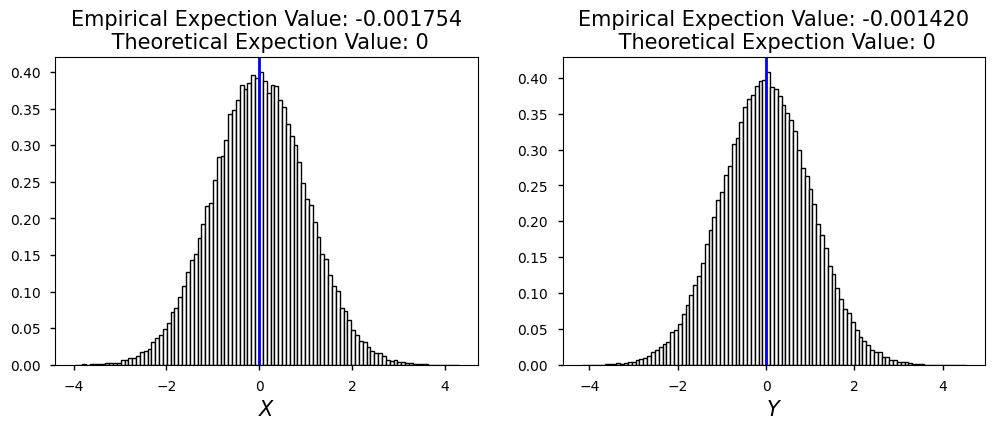
\includegraphics[width=0.9\textwidth]{images/nor_polar.png}
	\caption{Generating independent $X, Y \sim N(0,1)$ with polar method}
	\label{normal polar}
\end{figure}

